\chapter*{初高衔接}
\section{高中数学第一课}
\begin{center}
	原文来源:\citet{JiangGaoZhongShuXueDiYiKeDeJiaoXueGouXiang2016}
\end{center}

俗话说,好的开头是成功的一半.进入高中后,学生对每门课的第一节课都充满了期待.高中数学起始课应避免一上来就讲新课内容,可设计成“导游课”,像导游一样,每到一个景点时,先给游客对景点的特色、亮点、注意事项等作一个全貌的介绍.建议高中数学第一课可从两个方面进行构想:\textbf{一方面通过一些实例介绍高中数学之美妙,强调高中数学之重要,对初、高中数学特点进行比较;另一方面介绍高中数学的学习方法}.

\subsection{例说高中数学之美妙}
兴趣是最好的老师!要让学生喜欢数学,最有效的动力就是要激发学生学习数学的热情,让学生的内心能真正感受到数学之魅力,对高中数学充满渴望与期待!
\begin{example}[等势集合]
	请问:长度为1cm的线段上的点的个数与长度为2cm的线段上的点的个数哪个多?

	一部分学生认为2cm的线段上的点的个数多,并且是2倍关系,因为2cm线段的长是1cm线段长的2倍.但也有一部分学生会认为答案是一样多,因为都有无限个,无限就是一样的.

	后面一部分学生回答的答案是正确的,但理由是错误的,因为无限多不一定是一样多.这里可给学生介绍两个无限多元素是相等的需要两者能建立一一对应关系,这一点学生是容易接受的.可从学生与学号开始入手.再通过下图,即可明白.
	\begin{center}
		\tikzset{every picture/.style={line width=0.75pt}} %set default line width to 0.75pt        

		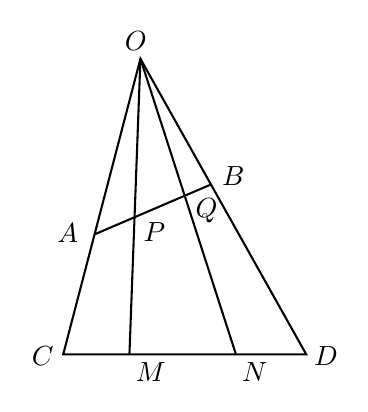
\begin{tikzpicture}[x=0.75pt,y=0.75pt,yscale=-1,xscale=1,scale=0.8]
			%uncomment if require: \path (0,300); %set diagram left start at 0, and has height of 300

			%Shape: Triangle [id:dp8404205470797059] 
			\draw   (322.17,54.17) -- (422,232.17) -- (275.67,232.17) -- cycle ;
			%Straight Lines [id:da9008684259134017] 
			\draw    (294.89,159.78) -- (364.89,129.78) ;
			%Straight Lines [id:da7092672100334034] 
			\draw    (322.17,54.17) -- (315.56,231.78) ;
			%Straight Lines [id:da3275050790851046] 
			\draw    (322.17,54.17) -- (379.56,231.78) ;

			% Text Node
			\draw (310.89,36.07) node [anchor=north west][inner sep=0.75pt]    {$O$};
			% Text Node
			\draw (270.22,151.73) node [anchor=north west][inner sep=0.75pt]    {$A$};
			% Text Node
			\draw (369.56,117.07) node [anchor=north west][inner sep=0.75pt]    {$B$};
			% Text Node
			\draw (254.89,225.73) node [anchor=north west][inner sep=0.75pt]    {$C$};
			% Text Node
			\draw (424.89,225.73) node [anchor=north west][inner sep=0.75pt]    {$D$};
			% Text Node
			\draw (317.56,235.18) node [anchor=north west][inner sep=0.75pt]    {$M$};
			% Text Node
			\draw (381.56,235.18) node [anchor=north west][inner sep=0.75pt]    {$N$};
			% Text Node
			\draw (322.22,151.07) node [anchor=north west][inner sep=0.75pt]    {$P$};
			% Text Node
			\draw (353.56,136.4) node [anchor=north west][inner sep=0.75pt]    {$Q$};


		\end{tikzpicture}
	\end{center}

	紧接着可问:

	(1)长度为1cm的线段上的点的个数与长度为100m的线段上的点的个数哪个多?

	(2)半径为1的圆周上点的个数与半径为2的圆周上点的个数哪个多?

	(3)正整数的个数与正偶数的个数一样多吗?

	(4)有理数与整数的个数一样多吗?

	(5)有理数与无理数的个数一样多吗?

	要告诉学生有理数与无理数是不一样多的,等到大学才能明白,这也是否定“无限多就是一样多的”的一个反例.
\end{example}
\begin{purpose}
	该例是高中第一章集合内容的拓展,通过该例让学生感悟到有限与无限之间有质的区别,在数学中部分可以等于整体,这在日常的生活中是不可思议的,因此本例是激发学生好奇心的很好素材.此外,希尔伯特旅馆的故事都可结合讲.
\end{purpose}
\begin{note}[希尔伯特旅馆\cite{XiErBoTeLuGuanBeiLun2023}]
	假设有一个拥有可数无限多个房间的旅馆,且所有的房间均已客满。或许有人会认为此时这一旅馆将无法再接纳新的客人(如同有限个房间的情况),但事实上并非如此。

	有限个新客人:设想此时有一个客人想要入住该旅馆。由于旅馆拥有无穷个房间,因而我们可以将原先在1号房间原有的客人安置到2号房间、2号房间原有的客人安置到3号房间,以此类推,这样就空出了1号房间留给新的客人。重复这一过程,我们就能够使任意有限个客人入住到旅馆内。

	无限个新客人:另外,我们还能使可数无限个新客人住到旅馆中:将1号房间原有的客人安置到2号房间、2号房间原有的客人安置到4号房间、n号房间原有的客人安置到2n号房间,这样所有的奇数房间就都能够空出来以容纳新的客人。
\end{note}

\begin{example}[杨辉三角]
	通过观察$(a+b),(a+b)^2,(a+b)^3,\ldots$ 展开式的各项系数,介绍杨辉三角.再尝试对 $(a+b)^5$ 的展开.
	\begin{equation*}
		\begin{array}{cccccccccc}
			  &   &   &   & 1      &   &   &   &   & \\
			  &   &   & 1 &        & 1 &   &   &   & \\
			  &   & 1 &   & 2      &   & 1 &   &   & \\
			  & 1 &   & 3 &        & 3 &   & 1 &   & \\
			1 &   & 4 &   & 6      &   & 4 &   & 1 & \\
			  &   &   &   & \cdots &   &   &   &   &
		\end{array}
	\end{equation*}
	本例是高中二项式定理中将介绍的杨辉三角(如图).杨辉三角又称贾宪三角形,帕斯卡三角形,是二项式系数在三角形中的一种几何排列.在欧洲,这个表叫做帕斯卡三角形.帕斯卡(1623—1662)是在1654年发现这一规律的,比杨辉要迟393年,比贾宪迟600年.
\end{example}
\begin{purpose}
	除展示数学结构美之外,渗透归纳思想,同时又渗透一下数学文化.
\end{purpose}

\begin{example}[极限雏形]
	当 $n \rightarrow \infty$ 时, $1+\frac{1}{2}+\frac{1}{3}+$ $\cdots+\frac{1}{n}$ 的值会不会超过 10?超过 100?超过 1 亿?

	有学生会认为超过 1 亿, 他相信积少成多的道理. 老师在肯定答案之时又马上给出变式: 当 $n \rightarrow \infty$时, $1+\frac{1}{2^2}+\frac{1}{3^2}+\cdots+\frac{1}{n^2}$ 的值会不会超过 10?超过 100? 超过 1 亿? 变化之后,连 2 都不会超过. 通过这种相似问题, 但结果又大相径庭, 从而引起学生的认知冲突, 从而激发学生对数学的探究欲望, 告诉学生,这些道理等以后学了极限就清楚了.
\end{example}
\begin{purpose}
	一让学生感受数列的收敛性和发散性, 二让学生再一次体会数学的奇异美.
\end{purpose}

\begin{example}[几何级数]
	电影《漂流瓶》中有一个故事,在船上有几位漂亮的女大学生,同时也有几位文化程度不高的男青年.在这些男青年中有一位绰号叫“三万”的,因为他有三兄弟,父母亲留给他们的财产共10万,平分后每人三万多点,故号称三万.其中一位女大学生想考考“三万”的才华,她说:“我跟你谈恋爱,有个条件:第1天给我1分钱,第2天给2分钱,第3天给4分钱,以后每天给的钱都是上一天的2倍.这样连续给一个月,如果给得起,我就同意.”而号称三万的青年认为这是毛毛雨,说可以,却不知道这是一个圈套.当用计算器按到第10天时,总共需要的钱只有10元2角4分,当按到第20天时,还行,1万多一点,而接下去就很快了,一个月下来给的钱总共大约需要2150多万.

	因为这个数列是成几何级数增长,增长速度之快是出乎人的常识之外.类似的还有折纸游戏,国王奖励国际象棋发明者的故事等等.
\end{example}
\begin{purpose}
	这个知识涉及到高中等比数列求和知识,另一点让学生明白知识的重要性.
\end{purpose}

\begin{example}[几何直觉]
	有两个三角形,其边长分别为17,25,26与17,25,28,求它们的内切圆半径谁大谁小.

	分析: 由 海 伦 公 式 $r=\sqrt{\frac{1}{p}(p-a)(p-b)(p-c)}, p=\frac{a+b+c}{2}$ 可算得: 以 $17,25,26$ 为边长的三角形的内切圆半径 $r_1=6$, 以 $17,25,28$ 为边长的三角形的内切圆半径 $r_2=6$.

	结果为 $r_1=r_2$, 完全出人意外! 估计百分之九十九的人会认为, 这两个三角形的内切圆半径虽然彼此相差不大, 但总应该有些微小差别, 绝对不会是相等的.
\end{example}
\begin{purpose}
	数学中直觉不一定可靠, 有时需要严密论证.
\end{purpose}

\begin{example}[数学悖论]
	一个理发师给自己立了这么一条店规:“只给那些不给自己刮脸的人刮脸.”那么,这位理发师的脸该不该由他自己刮?

	如果理发师的脸由他自己刮,则他属于“自己给自己刮脸的人.”因此,理发师不应该给自己刮脸;如果理发师的脸不由他自己刮,则他又属于“自己不给自己刮脸的人.”因此,他的脸可由自己刮,这显然又与上述“自己不给自己刮脸的人”相矛盾.从以上分析,这样不对,那样也不对,就是数学中的悖论.
\end{example}
\begin{purpose}
	激发学生对数学逻辑的兴趣,同时也可介绍数学发展的几次危机.
\end{purpose}
\begin{note}[数学危机\cite{ShuXueWeiJi2023}]
	数学危机在历史上发生过三次,每一次均对数学的发展有重大影响。在第一次数学危机中,因为发现腰长为1的等腰直角三角形的斜边长度无法写成有理数,从而引申出日后的无理数概念。第二次数学危机得以解决微积分引入无穷小量而产生的问题。第三次数学危机则是因罗素悖论而起,它点出朴素集合论中的缺失。
\end{note}
\subsection{例说高中数学之重要}
做一件事光有兴趣是远远不够的,只有认识到做这件事的意义和重要性,才能有做好这件事不竭的动力,学习数学也是一样.数学学科是一门基础学科,它的重要性是多方面、多角度、多层次的.

1. 数学是一种描述自然的语言.

数学语言刻画事物的数量关系、形式与形状,反映事物的本质属性.当人们需要把客观事物的认识精确化的时候,必须使用数学语言. 诺贝尔物理学奖获得者菲曼曾说:“要是没有数学语言,宇宙几乎是不可描述的!”例如,牛顿用数学公式展示了物质运动的三大定律,爱因斯坦用黎曼有关弯曲空间曲率理论阐述广义相对论;化学家、生物学家、经济学家等都必须用数学语言使自己的学科精密化.

2.数学是培养思维能力的重要载体.

法国数学家格瑞斯曼说过这样的话:“数学除了锻炼敏锐的理解力,发现真理外,它还有另一个训练全面考虑和科学系统的头脑的开发功能.”

通过数学学习,形成一种数学思想和能力,明确数量观念,注意事物的数量关系与变化规律;通过数学学习,了解数学的概念、方法、理论等的产生和发展的渊源及过程,了解和领会从实际出发建立数学模型,再到解决问题的全过程;通过数学学习,提高人的逻辑思维能力,能在纷繁复杂的各项工作面前有条不紊地处理等.

\begin{example}
	甲、乙二人在一圆形桌面上轮流放面值一样的硬币,不可重叠,当谁放不下了,谁就输.如果甲先放,问有无必胜的策略?
\end{example}

\begin{analysis}
	如果甲、乙二人随意去放,显然甲不一定能赢.但如果能从数学对称原理去想,先放者就有必胜的策略.只要甲第一次先放在桌子的中心,接下来乙放,然后甲放在乙刚放的关于圆心的对称点上,依次下去,由对称原理,只要乙能放,甲肯定能放,故甲胜.

	本题将随意放硬币的游戏进行有序化,先夺取“战略高地”,这就是数学的思维.
\end{analysis}

\begin{example}
	证明: 任意6人中,至少有3人两两相互认识或两两互不认识.
\end{example}

\begin{analysis}
	这一问题如果将各种情况都加以考虑,也是一种思路,穷举法,但情况比较多,显得繁杂.现在将问题进行数学化,就不难了.将6人视为平面上6个点,相互认识的用实线相连,相互不认识的用虚线相连.

	先考虑从A点出发与其它五个点连线情况,共有5条线,由于只有实线与虚线二种情形,因此由抽屉原理可以断定这5条线中至少有3条是同一类型的,譬如,有3条实线AB,AC,AE,现在分析B,C,E三点之间的连线,若B,C,E三点之间的连线有一条是实线,譬如BE,那么A,B,E三者的连线都是实线,问题解决,反之,若B,C,E三点之间的连线都是虚线,问题也得证.
\end{analysis}

3.数学是科学技术进步的直接推手

我国著名数学家华罗庚先生曾说:“宇宙之大,粒子之微,火箭之速,化工之巧,地球之变,生物之谜,日用之繁等各个方面,无处不有数学.”由此可见数学应用是非常广泛的.

二十世纪科学技术进步给人类生产和生活带来的巨大变化确实令人赞叹不已.从远古时代起一直是人们幻想的“顺风耳”、“千里眼”、“空中飞行”和“飞向太空”都在这一世纪成为现实.回顾二十世纪的重大科学技术进步,以下几个项目无疑是影响最大的,而数学的预见和推动作用是非常关键.

(1)先有了麦克斯韦方程,人们从数学上论证了电磁波,其后赫兹才有可能做发射电磁波的实验,接着才会有电磁波声光信息传递技术的发展.

(2)爱因斯坦相对论的质能公式首先从数学上论证了原子反应将释放出的巨大能量,预示了原子能时代的来临.随后人们才在技术上实现了这一预见,到了今天,原子能已成为发达国家电力能源的主要组成部分.

(3)牛顿当年已经通过数学计算预见了发射人造天体的可能性,差不多过了将近三个世纪,人们才实现了这一预见.

(4)电子数字计算机的诞生和发展完全是在数学理论的指导下进行的.数学家图灵和冯诺依曼的研究对这一重大科学技术进步起了关键性的推动作用.

(5)遗传与变异现象虽然早就为人们所注意.生产和生活中也曾培养过动植物新品种.遗传的机制却很长时间得不到合理解释,十九世纪60年代,孟德尔以组合数学模型来解释他通过长达8年的实验观察得到的遗传统计资料,从而预见了遗传基因的存在性.多年以后,人们才发现了遗传基因的实际承载体,到了本世纪50年代沃森和克里发现了DNA分子的双螺旋结构.这以后,数学更深刻地进入遗传密码的破译研究.

数学是人类理性思维的重要方式,数学模型,数学研究和数学推断往往能作出先于具体经验的预见.这种预见并非出于幻想而是出于对以数学方式表现出来的自然规律和必然性的认识,随着科学技术的发展,数学、预见的精确性和可检验性日益显示其重意义.

\subsection{高中数学与初中数学的差异}
1. 知识差异

初中: 内容少、浅、面窄,常量为主, 题型少、简单,可反复磨炼,甚至死记硬背就可以考出高分.

高中:知识多、深、面宽;变量为主, 题型多, 没有时间反复.

2. 教法差异

初中: 课堂容量小,讲速慢,题型少,反复,模仿.

高中: 课堂容量大,知识复杂,速度快,题型多,很少反复.

3. 学法差异

初中: 自学能力差, 讲授, 被动学, 反复练.

高中:自主探索, 主动学习, 获得知识的渠道宽.

4.语言差异

初中:初中的数学主要是以形象、通俗的语言方式进行表达.

高中: 高一进来就触及抽象的集合符号语言、逻辑运算语言、函数语言、图形语言等, 也就是说抽象化程度大大提升,抽象是感觉难的主要原因.

5.思维差异

初中:很多老师为学生将各种题型建立了统一的思维模式(如:解分式方程分几步;因式分解先看什么、再看什么,等等),确定了常见的思维套路,因此,形成初中阶段在数学学习中习惯于这种机械的、便于操作的定式.

高中:在解题方法步骤上灵活多变,往往能一题多解,用代数法能解出,用几何法也能解出,但每种解题方法所用时间和出错的机会不一样,这就要求对各种思想方法如数形结合、分类讨论、整体换元、消元等思想方法融会贯通,思想方法的学习就像外语的语法一样,在高中数学的学习中占很大比例.

\subsection{高中数学学习方法}
(一)高中数学的学习方法六字方针:思考,运算,积累.

1.思考是核心.

学数学有时课堂上都能听懂,老师讲的题目觉得自己都会,可是课下自己一做就错,有的问题甚至没有思路.学数学最忌讳的是老师讲同学听,听完之后做笔记,从头听到尾,从头记到尾,听的特明白,笔记记得特清楚,轮到自己一做题还是不会做,还是无处下手,这就好比同学们站在岸上学游泳,没有经过那个被水淹、在水里扑腾的过程,老师示范的再清楚你还是白搭.要将思考贯穿于数学学习的整个过程,无论课上老师的提问,还是课下自己做题,我们始终要做的就是思考:为什么这样做,为什么要这样变形,这道题还能怎么做,这类题目解决的共同方法是什么,所蕴含的思想方法是什么,等等.数学学习的主阵地是课堂,老师提出问题后同学们的大脑就要飞速地旋转,哪怕有一点点思路也要积极回答,这样积极参与的过程学习效率很高.

2.运算是基础.

数学离不开算.在小学阶段被称为算术,初中阶段被称为代数,用字母代替数字进行运算,在高中更是通过指数、对数、三角函数、向量、排列组合、算法等载体发展人的计算能力.较复杂的解析几何题目运算过程可达几十步,只要错了一个正负号或算错一个小数就会满盘皆输,整个大题报废,离开了一个强大的计算能力就谈不上学好数学.所以说,一道题从有了思路到完整解答还差多少里?十万八千里!为了提高计算能力,在笔算的基础上更要心算.学数学要将算放在首位,这也是对数学的第一个也是最重要的一项要求.运算是能力,能力的提升没有什么巧妙的方法,就是要拿出你的耐心和细心大量地练,亲自动手将每一个得数算出来,当然还要掌握好算理.

3.积累是保障.

数学课如果有几节课没听,有几节练习没跟着做,再接着听便不好听懂,甚至一点都不会.由此可见数学的一个重要特点就是必须将先学的知识彻底掌握才能进行后续的学习.前边提到数学的一个重要特点就是抽象,内容都是用字母和符号表达的,这就要求同学们必须对学过的东西进行持之以恒的反复记忆和运算,通过这种方式将抽象的东西内化,最后形成直觉.但数学题太多了,人们都把它比喻成题海,都记不把人累死吗?这就涉及到积累什么东西的问题.牵牛要牵鼻子,想问题办事情要抓关键,抓主要矛盾.高中数学的这个关键就是指好题:有代表性的,通过这道题能掌握好几个重要知识点,能掌握解一类问题的通法,能以一顶十的题目.要是让你单纯背诵你总觉得这事有点荒唐,不像文科的东西那样好背,或者说根本就不适合背诵,怎么办?多做,好题做六遍,做的遍数多自然就掌握了.所以我们要积累的东西是上课老师所讲授的典型例题,解决典型例题的思想方法.课上要逐渐学会迅速记录简明的课堂笔记,课下详细整理,补充详实.除此之外还有学着整理做过的试卷,这些试卷上往往有很多精彩的题目,都往笔记本上誊写没那时间,索性直接将笔记做在卷子上,每隔一段时间进行阅读,尤其是考前这么做效果最好.

(二)五点建议

1.认真听好每一节课

有的同学上课不听,下课不看,资料不做,考试前拿着课本在那记公式,总结知识点,考试成绩是一塌糊涂.原因是什么?为什么初中可以考前突击,现在却不行了?初中知识简单,结构单一,高中数学灵活多变,不是靠死记硬背,更多的是课堂上讲解的解题的思想方法.

2.做好数学笔记

特别是对概念不同侧面的理解,以及典型例题.

3. 建立数学错题本

把平时容易出现错误的知识或推理记载下来,以防再犯.争取做到:找错、析错、改错、防错.达到:能从反面入手深入理解;能由果溯因把错误原因弄个水落石出、以便对症下药;解答问题完整、推理严密.

4. 记忆数学规律和数学小结论

高中数学不是靠死记硬背,但是不代表不背,基本的规律和结论还是必须记的,记的熟练了,自然也就能灵活运用了.

5. 学会总结归类

(1)从数学思想分类;(2)从解题方法归类;(3)从知识应用上分类.

\begin{note}
	个人按照时间顺序的三点建议:
\begin{enumerate}
	\item     课前——做好预习,提前阅读教材并完成全品“课前预习”部分,了解将要学习的内容,不懂的地方做好标记,带着问题上课;
	\item 课堂——集中精力听讲,积极参与课堂讨论,及时记笔记。对于不理解的部分,课后及时解决;
	\item 课后——及时复习当天内容,先自己复习梳理一遍当天所学知识再写作业,按时提交作业,建立数学错题本,学会总结归纳.
\end{enumerate}
\end{note}

本文从四个方面设计高中数学起始课,由于内容多,建议用两种方式灵活处理,一是上两节课;二是精简内容,并结合教师自己的特长与兴趣进行设计.
